\documentclass{article}

\usepackage{ipprocess}
%\usepackage{lmodern}
\usepackage{longtable}
\usepackage[utf8]{inputenc} 
\usepackage[T1]{fontenc}
\pagestyle{fancy}
\usepackage{libertine}
\usepackage{epstopdf}

%\usepackage[author={João Carlos Nunes Bittencourt}]{pdfcomment}

\sloppy

\title{32-bit $\mu$DLX Core Processor}

\graphicspath{{./pictures/}} % DiretTBDrio padrTBDo de figuras.
\makeindex
\begin{document}
  \capa{1.0}{abril}{2014}{32-bit $\mu$DLX Core Processor}{Architecture Specification}{Universidade Federal da Bahia}
  \newpage

%%%%%%%%%%%%%%%%%%%%%%%%%%%%%%%%%%%%%%%%%%%%%%%%%%
%% GNU LGPL Licence
%%%%%%%%%%%%%%%%%%%%%%%%%%%%%%%%%%%%%%%%%%%%%%%%%%

  
\begin{center}
\begin{Large}\textbf{GNU LGPL License}                          \end{Large}
\end{center}
\vspace{2cm}
\fbox{
  \parbox{.7\textwidth}{
    \vspace{0,5cm}
    \begin{scriptsize}
    This file is part of uDLX (micro-DeLuX) soft IP-core.\\

    uDLX is free soft IP-core: you can redistribute it and/or modify
    it under the terms of the GNU General Public License as published by
    the Free Software Foundation, either version 3 of the License, or
    (at your option) any later version.\\

    uDLX soft core is distributed in the hope that it will be useful,
    but WITHOUT ANY WARRANTY; without even the implied warranty of
    MERCHANTABILITY or FITNESS FOR A PARTICULAR PURPOSE. See the
    GNU General Public License for more details.

    You should have received a copy of the GNU General Public License
    along with uDLX. If not, see <http://www.gnu.org/licenses/>.
    \end{scriptsize}
    \vspace{0,5cm}
  }
}

\newpage

%%%%%%%%%%%%%%%%%%%%%%%%%%%%%%%%%%%%%%%%%%%%%%%%%%
%% Revision History
%%%%%%%%%%%%%%%%%%%%%%%%%%%%%%%%%%%%%%%%%%%%%%%%%%
  \section*{\center Revision History}
  \vspace*{1cm}
  \begin{table}[ht] % aqui comeTBDa o ambiente tabela
  \centering
  \begin{tabular}[pos]{|m{2cm} | m{7.2cm} | m{3.8cm}|} 
  \hline % este comando coloca uma linha na tabela
  \cellcolor[gray]{0.9}
  \textbf{Date} & \cellcolor[gray]{0.9}\textbf{Description} & \cellcolor[gray]{0.9}\textbf{Author(s)}\\ \hline
  \hline
  \small 04/27/2014 & \small Conception & \small João Carlos Bittencourt \\ \hline
  \small 04/30/2014 & \small Instruction layout description & \small João Carlos Bittencourt \\ \hline
  \small 05/09/2014 & 
  \begin{small}
    \begin{itemize}
      \item Text revision;
      \item Update diagrams and instruction layout;
      \item Update instruction fetch I/O definitions;
      \item Missing pictures inclusion;
      \item Include memory access and write back pin/port definitions;
    \end{itemize}
  \end{small} & \small João Carlos Bittencourt \\ \hline
  \small 04/13/2014 & \small Missing pictures & \small João Carlos Bittencourt \\ \hline
  \small 04/15/2014 & \small   \begin{small}
    \begin{itemize}
      \item Fix instruction fetch pin definitions;
      \item Include instruction fetch datapath;
      \item Include pipeline registers definitions;
      \item Fix memory access stage pin/port definitions;
      \item Include write back data path;
    \end{itemize}
  \end{small} & \small João Carlos Bittencourt \\ \hline
  \small 04/15/2014 & \small Add execute block diagram & \small Igo Amauri Luz \\ \hline
  \small 04/16/2014 & \small   \begin{small}
    \begin{itemize}
      \item Add branch prediction signal to ID and IF blocks and pin definitions;
      \item Add table for pin definitions in Execute stage
      \item Add branch prediction signal in pipeline registers definitions;
      \item Include architecture interface figure;
    \end{itemize}
  \end{small} & \small João Carlos Bittencourt \\ \hline 
  \small 04/18/2014 & \small Add execute datapath diagram & \small Igo Amauri Luz \\ \hline
  \small 04/23/2014 & \small Formating; Stakeholders listing & \small João Carlos Bittencourt \\ \hline  
  \end{tabular}
  \end{table}

  \newpage
  
  \tableofcontents
  \newpage

%%%%%%%%%%%%%%%%%%%%%%%%%%%%%%%%%%%%%%%%%%%%%%%%%%
%% Concent
%%%%%%%%%%%%%%%%%%%%%%%%%%%%%%%%%%%%%%%%%%%%%%%%%%
  \section{Introduction}
  \subsection{Purpose}
  The main purpose of this document is to define specifications of a uDLX implementation and to provide a full overview of the design. This specifications defines all implementation parameters that composes the general uDLX requirements and specification. This definitions include processor operation modes, instruction set (ISA) and internal registers characteristics. This document also include detailed information of pipeline stages architecture, buses and other supplemental units.

  \subsection{Stakeholders}
  \FloatBarrier
  \begin{table}[H] 
    \begin{center}
      \begin{tabular}[pos]{|m{5cm} | m{8cm}|} 
        \hline % este comando coloca uma linha na tabela
        \cellcolor[gray]{0.9}\textbf{Name} & \cellcolor[gray]{0.9}\textbf{Roles/Responsibilities} \\ \hline
        Igo Amauri Luz & TBD \\ \hline
        João Carlos Bittencourt & TBD \\ \hline  
        Lauê Rami Costa & TBD \\ \hline
        Linton Thiago Esteves & TBD \\ \hline  
        Victor Valente & TBD \\ \hline
      \end{tabular}
    \end{center}
  \end{table}    
  
  \subsection{Document Outline Description}
  This document is outlined as follow:
	
	\begin{itemize}
	  \item Section \color{black}{\ref{sec:architecture_overview}}: This section presents the core processor block diagram, Pin/Port definitions and global parameters and configuration directives.
	  \item Section \color{black}{\ref{sec:instruction_layout}}: This section presents the $\mu$DLX instruction layout and specifications. 
    \item Section \color{black}{\ref{sec:architecture_description}}: This section presents a description of each pipeline stage block, including pin definitions, signals and internal datapath.
	\end{itemize}
		
  \subsection{Acronyms and Abbreviations}
  Along this and other documents part of this project, it will be recurrent the usage of some acronyms and abbreviations. In order to keep track of this elements the Table \ref{tab:definitions} presents a set of abbreviations used and its corresponding meaning.
  
  \FloatBarrier
  \begin{table}[H]
    \begin{center}
      \caption{Acronym and descriptions of elements in this document.}
      \label{tab:definitions}

      \begin{tabular}[pos]{|m{2cm} | m{9cm}|} 
	\hline % este comando coloca uma linha na tabela
	\cellcolor[gray]{0.9}\textbf{Acronym} & \cellcolor[gray]{0.9}\textbf{Description} \\ \hline
	RISC & Reduced Instruction Set Computer \\ \hline
	GPR & General Purpose Registers \\ \hline
	FPGA & Field Gate Programmable Array \\ \hline
	GPPU & General Purpose Processing Unit \\ \hline
	SDRAM & Synchronous Dynamic Random Access Memory\\ \hline
	HDL & Hardware Description Language \\ \hline
	RAW & Read After Write \\ \hline
	CPU & Central Processing Unit \\ \hline
	ISA & Instruction Set Architecture \\ \hline
	ALU & Arithmetic and Logic Unit \\ \hline
	PC  & Program Counter \\ \hline
	RFlags & Flags Register \\ \hline
	Const  & Constant \\ \hline
  BPM    & Branch Prediction Buffer \\ \hline
      \end{tabular}
    \end{center}
  \end{table}
  
  \newpage
  \section{Architecture Overview}
  \label{sec:architecture_overview}
  
  \subsection{Interface Architecture}
  The $\mu$DLX architecture interface is composed by the following components.
  \begin{itemize}
    \item \textbf{$\mu$DLX 32-bit Core:} The core four-deep pipeline processor.
    \item \textbf{Memory Interface:} Provides a middle layer between the core processor and the external memories. This interface also controls the bootloader process.
    \item \textbf{SDRAM Controller:} Provides the interface for controlling the external SDRAM.
    \item \textbf{SRAM Controller:} Provides the interface for controlling the external SRAM.
  \end{itemize}
  \begin{figure}[H]
    \centering
    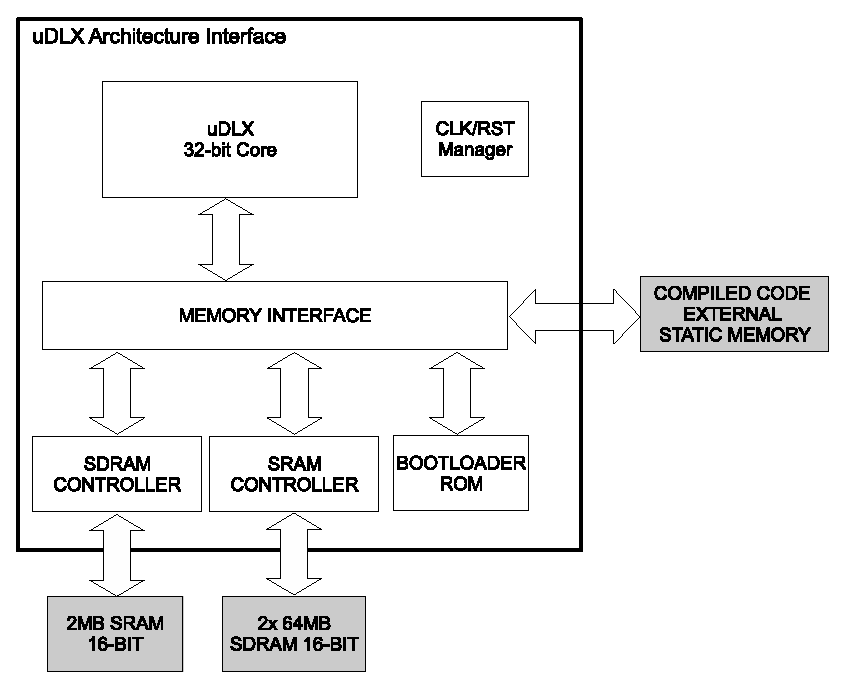
\includegraphics[width=.8\linewidth]{pictures/architecture_interface.eps}
  \end{figure}

  \subsection{Block Diagram}
  \begin{figure}[H]
    \centering
    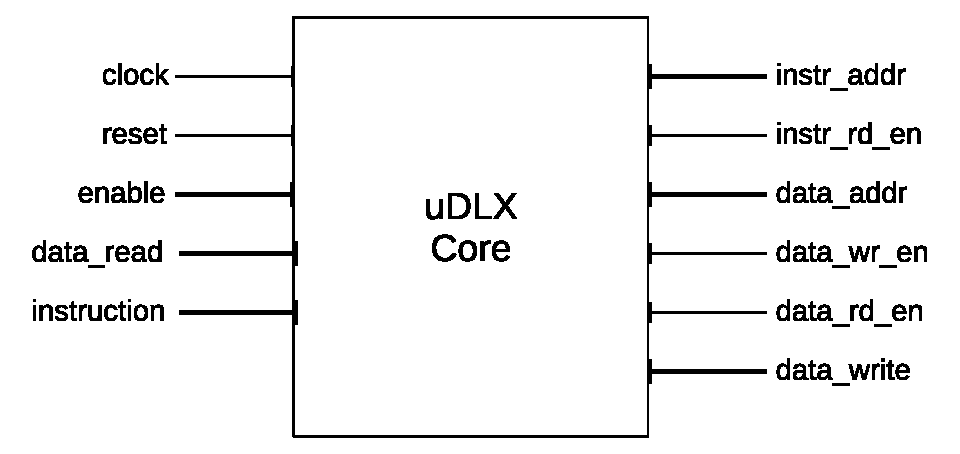
\includegraphics[width=.85\linewidth]{pictures/udlx_block.eps}
  \end{figure}
 
 
  \subsection{Pin/Port Definitions}
  \FloatBarrier
  \begin{table}[H]
    \begin{center}
      \begin{tabular}[pos]{| l | c | c | m{7cm} |} \hline 	
      \multicolumn{1}{|c|}{\cellcolor[gray]{0.9}\textbf{Name}} & 
      \multicolumn{1}{c|}{\cellcolor[gray]{0.9}\textbf{Length}} & 
      \multicolumn{1}{c|}{\cellcolor[gray]{0.9}\textbf{Direction}} &
      \multicolumn{1}{c|}{\cellcolor[gray]{0.9}\textbf{Description}} \\ \hline
	 clock 		& 1 	& input 	& CPU core clock  	\\ \hline
	 reset 		& 1	& input		& CPU core reset  	\\ \hline
	 instruction 	& 32	& input 	& SRAM instruction data \\ \hline
	 data\_read 	& 32	& input 	& SDRAM read data \\ \hline
	 instr\_addr 	& 20	& input 	& SRAM address \\ \hline
	 instr\_rd\_en 	& 1	& output 	& SRAM read enable  \\ \hline
	 data\_addr 	& 13	& output	& SDRAM address \\ \hline
	 data\_wr\_en 	& 1	& output 	& SDRAM write enable  \\ \hline
	 data\_rd\_en 	& 1	& output 	& SDRAM read enable  \\ \hline
   data\_write   & 32 & output  & SDRAM write data  \\ \hline
      \end{tabular}
    \end{center}
  \end{table}  
   
  \subsection{Parameters and Configurations}

 \FloatBarrier
  \begin{table}[H]
    \begin{center}
      \begin{tabular}[pos]{| l | l | m{8cm} |} \hline 	
      \multicolumn{1}{|c|}{\cellcolor[gray]{0.9}\textbf{Name}} & 
      \multicolumn{1}{c|}{\cellcolor[gray]{0.9}\textbf{Value}} & 
      \multicolumn{1}{c|}{\cellcolor[gray]{0.9}\textbf{Description}} \\ \hline
	  & &  	\\ \hline
      \end{tabular}
    \end{center}
  \end{table} 
    
  \newpage
  \section{Instructions Layout}
  In order to be the most close to the DLX and also be as compatible as possible to MIPS R2000 and R3000 architecture few instructions were added to the instruction set. Instructions that are not present in DLX and MIPS architecture are added in not used OPCODES.
  \label{sec:instruction_layout}

  \subsection{Instructions Set}
  DLX instruction structure has 5 types of instructions, the floating point instructions were removed. The 3 DLX instructions types supported in the project are shown in figure below.
  
  \begin{figure}[H]
    \centering
    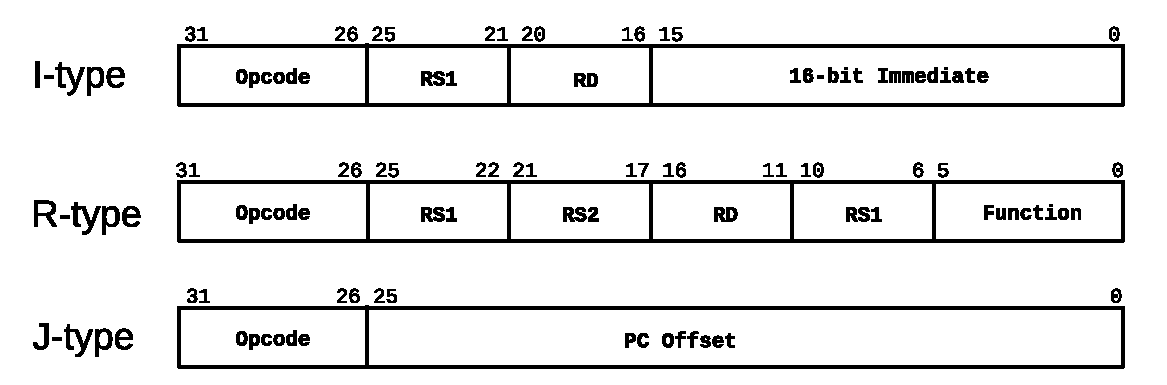
\includegraphics[width=\linewidth]{pictures/instruction_set.eps}
  \end{figure} 
  
NOP instruction has zero in all bits and will not be mapped to an instruction type.
  
  \subsection{I-type Instruction}
  Immediate instructions use the immediate data to address a load and store operation, make arithmetic operations and make brachs using 
Some arithmetic immediate instructions were added because they make easier assembly programming. The conditional branch operations BEQZ and BNEQZ were added to enable some compiler compatibility and future core improvement.

  \FloatBarrier
  \begin{table}[H]
    \begin{center}
      \begin{tabular}[pos]{| c | l | l |} \hline 	
      \multicolumn{1}{|c|}{\cellcolor[gray]{0.9}\textbf{OPCODE}} & 
      \multicolumn{1}{c|}{\cellcolor[gray]{0.9}\textbf{Mneumonic}} & 
      \multicolumn{1}{c|}{\cellcolor[gray]{0.9}\textbf{Operation}} \\ \hline
	 100011/0x23 	& lw & $R_D = mem$ \\ \hline
	 101011/0x2b 	& sw & $mem = R_D$ \\ \hline
	 101010/0x2A 	& brfl & $TBD$ \\ \hline
	 001000/0x08 & addi & $R_D = R_S1 + Sext(imm)$ \\ \hline
	 001010/0x10 & subi & $R_D = R_S1 - Sext(imm)$ \\ \hline
	 001101/0x12 & andi & $R_D = R_S1 \land Sext(imm)$ \\ \hline
	 001101/0x13 & ori & $R_D = R_S1 \lor Sext(imm)$ \\ \hline
	 000100/0x04 & beqz & $PC = PC + 4 +(R_S1 = 0~?~SExt(imm): 0)$ \\ \hline
	 000101/0x05 & bnez & $Fixme$ \\ \hline
	 000111/0x16 & jr & $PC = R_S1$ \\ \hline
      \end{tabular}
    \end{center}
  \end{table} 

Only LW, SW, BRFL, and JR instructions are in the p?oject requirements, the other were added to make compatibility and some codes easier.
  
  \subsection{R-type Instruction}
This instructions realize registers operations, most operations are arithmetic. All arithmetic opcodes are zero, differing only in the function value.

  \FloatBarrier
  \begin{table}[H]
    \begin{center}
      \begin{tabular}[pos]{| c | l | l |} \hline 	
      \multicolumn{1}{|c|}{\cellcolor[gray]{0.9}\textbf{OPCODE}} & 
      \multicolumn{1}{c|}{\cellcolor[gray]{0.9}\textbf{Mneumonic}} & 
      \multicolumn{1}{c|}{\cellcolor[gray]{0.9}\textbf{Operation}} \\ \hline
	 100000/0x20 	& add & $R_D = R_S1 + R_S2$ \\ \hline
	 100010/0x22 	& sub & $R_D = R_S1 - R_S2$ \\ \hline
	 100100/0x24 	& and & $R_D = R_S1 \land R_S2$ \\ \hline
	 100101/0x25 & or & $R_D = R_S1 \lor R_S2$ \\ \hline
	 011000/0x18 & mult & $R_D = R_S1 ~.~ R_S2$ \\ \hline
	 011010/0x1A & div & $R_D = R_S1 ~/~ R_S2$ \\ \hline
	 011100/0x1C & cmp & $R_D = R_S1 ~cmp~ R_S2$ \\ \hline
	 011101/0x1D & not & $R_D = \lnot R_S2$ \\ \hline

      \end{tabular}
    \end{center}
  \end{table} 

The MULT, DIV, CMP, and NOT instructions were added in DLX instruction set

  \subsection{J-type Instruction}
Instructions related with instruction memory jump. The instructions are JPC (J),RET (RFE), CALL (TRAP).
  \FloatBarrier
  \begin{table}[H]
    \begin{center}
      \begin{tabular}[pos]{| c | l | m{9cm} |} \hline 	
      \multicolumn{1}{|c|}{\cellcolor[gray]{0.9}\textbf{OPCODE}} & 
      \multicolumn{1}{c|}{\cellcolor[gray]{0.9}\textbf{Mneumonic}} & 
      \multicolumn{1}{m{9cm}|}{\cellcolor[gray]{0.9}\textbf{Operation}} \\ \hline
	 000010/0x02 	& jpc(j) & PC = PC + 4 \\ \hline
	 111110/0x3e 	& call(trap) & 
   trap = 1; \newline EPC = PC; \newline PC = SISR;
   \newline ESR = SR; \newline ECA = masked CA; \newline SR = 0; 
   \newline EDATA = SExt(imm); \newline Clear CA but catch new interrupt events \\ \hline
	 111111/0x3f 	& ret(rfe) & SR = ESR; \newline PC = EPC \\ \hline

      \end{tabular}
    \end{center}
  \end{table} 

%  \subsection{Control Transfer}
%  The $\mu$DLX core processor has five control transfer instructions encoded using the following three types. The first encoding type is used for unconditional jump and subroutine call. The second one is used for conditional branch, based on ALU flags. The third one reffers to the unconditional jump related to PC by an immediate value offset.
%
%  \hspace{-36px}\textbf{Type I}
%  \begin{figure}[H]
%    \centering
%    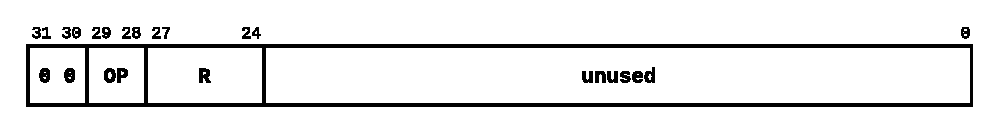
\includegraphics[width=\linewidth]{pictures/control_type_1.eps}
%  \end{figure}  
%  
%  \hspace{-36px}\textbf{Type II}
%  \begin{figure}[H]
%    \centering
%    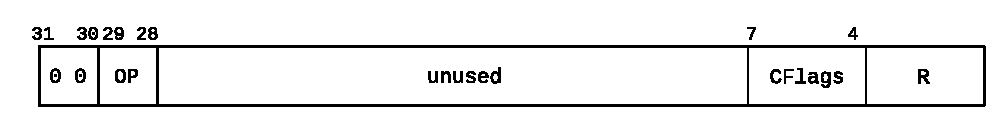
\includegraphics[width=\linewidth]{pictures/control_type_2.eps}
%  \end{figure}  
%  
%  \hspace{-36px}\textbf{Type III}
%  \begin{figure}[H]
%    \centering
%    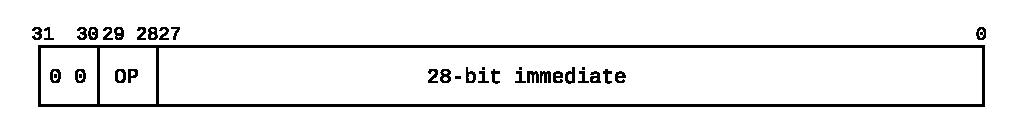
\includegraphics[width=\linewidth]{pictures/control_type_3.eps}
%  \end{figure}  
%  
%  \FloatBarrier
%  \begin{table}[H]
%    \begin{center}
%      \begin{tabular}[pos]{| c | l | l | l |} \hline 	
%      \multicolumn{1}{|c|}{\cellcolor[gray]{0.9}\textbf{Type}} & 
%      \multicolumn{1}{c|}{\cellcolor[gray]{0.9}\textbf{OP}} & 
%      \multicolumn{1}{c|}{\cellcolor[gray]{0.9}\textbf{Opperation}} &
%      \multicolumn{1}{c|}{\cellcolor[gray]{0.9}\textbf{Mnemonic}} \\ \hline
%	 I 	& 00 & Jump Register	& jr r \\ \hline
%	 I 	& 01 & Subroutine call  & call r \\ \hline
%	 II 	& 10 & Branch flags 	& brfl r, const\\ \hline
%	 III 	& 11 & Jump PC 		& jpc destiny\\ \hline	 
%      \end{tabular}
%    \end{center}
%  \end{table}   
%  
%  \subsection{Memory}
%  \begin{figure}[H]
%    \centering
%    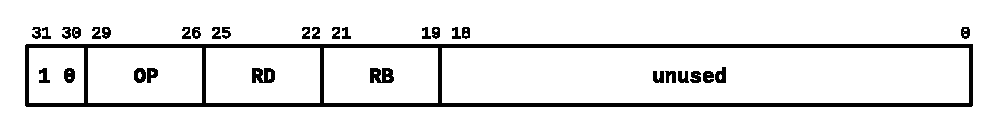
\includegraphics[width=\linewidth]{pictures/alu_instruction.eps}
%  \end{figure} 
%  
%  \FloatBarrier
%  \begin{table}[H]
%    \begin{center}
%      \begin{tabular}[pos]{| c | l | l |} \hline 	
%      \multicolumn{1}{|c|}{\cellcolor[gray]{0.9}\textbf{OP}} & 
%      \multicolumn{1}{c|}{\cellcolor[gray]{0.9}\textbf{Opperation}} & 
%      \multicolumn{1}{c|}{\cellcolor[gray]{0.9}\textbf{Mnemonic}} \\ \hline
%	 1000 & $R_D = Mem[R_B]$ 	& load d, b 	 \\ \hline
%	 1100 & $Mem[R_B] = R_D$ 	& store b, d 	\\ \hline
%      \end{tabular}
%    \end{center}
%  \end{table}   
  
  \section{Architecture Description}
  \label{sec:architecture_description}

  \subsection{Instruction Fetch}
  \subsubsection{Block Diagram}
  \begin{figure}[H]
    \centering
    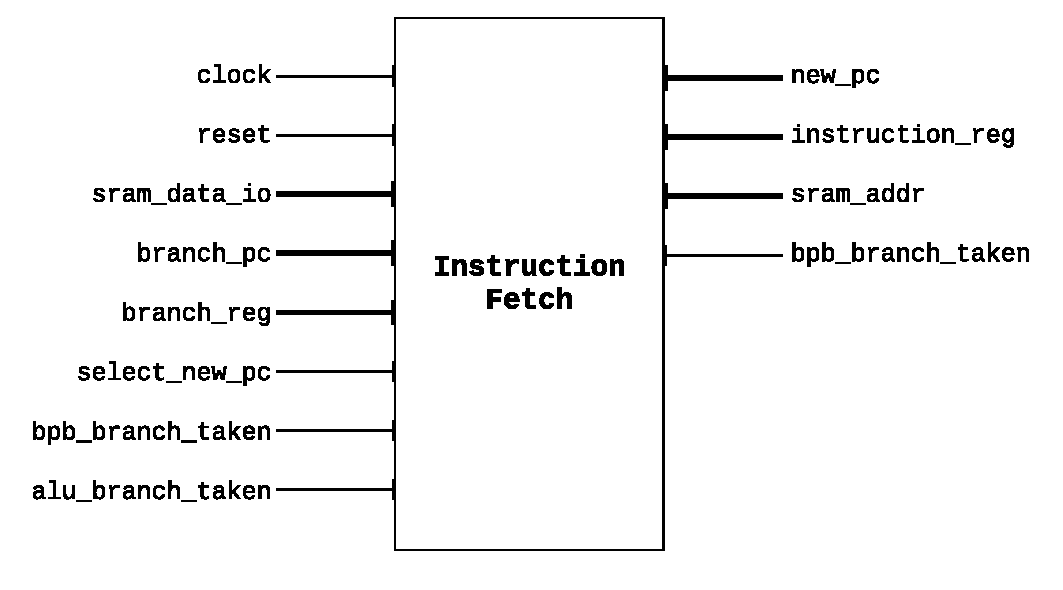
\includegraphics[width=\linewidth]{pictures/blocks/if_block.eps}
  \end{figure}    
  
  \subsubsection{Pin/Port Definitions}
  \FloatBarrier
  \begin{table}[H]
    \begin{center}
      \begin{tabular}[pos]{| l | c | c | m{7cm} |} \hline 	
      \multicolumn{1}{|c|}{\cellcolor[gray]{0.9}\textbf{Name}} & 
      \multicolumn{1}{c|}{\cellcolor[gray]{0.9}\textbf{Length}} & 
      \multicolumn{1}{c|}{\cellcolor[gray]{0.9}\textbf{Direction}} &
      \multicolumn{1}{c|}{\cellcolor[gray]{0.9}\textbf{Description}} \\ \hline
	 clock\_in 		          & 1 	& input 	& CPU core clock  	\\ \hline
	 reset\_in 		          & 1	  & input		& CPU core reset  	\\ \hline
	 inst\_mem\_data\_in     & ???	& input 	& SRAM data \\ \hline
	 %branch\_pc 	      & 20	& input 	& Branch address PC relative \\ \hline
	 %branch\_reg 	      & 20	& input 	& Branch address loaded from registers \\ \hline
     select\_new\_pc\_in    & 1   & input   & Signal used for branch not taken \\ \hline
     new\_pc\_in    & 20   & input   & New value of PC \\ \hline
   
	 new\_pc\_out 		        & 20	& output 	& Updated value of PC \\ \hline
	 instruction\_reg\_out 	      & 32	& output 	& CPU core instruction  \\ \hline
	 inst\_mem\_addr\_out 	      & 20	& output	& SRAM address \\ \hline
      \end{tabular}
    \end{center}
  \end{table} 

  \subsubsection{Internal Datapath} 
  The internal data path is composed by the following components.

  \begin{description}
    \item [Program Counter]: During the instruction time of an instruction this is the
address of the instruction word. The address of the instruction that occurs during
the next instruction time is determined by assigning a value to PC during an instruction time. If no value is assigned to PC during an instruction time by any pseudocode statement, it is automatically incremented by 2 before the next
instruction time.

  \end{description}

  \begin{figure}[H]
    \centering
    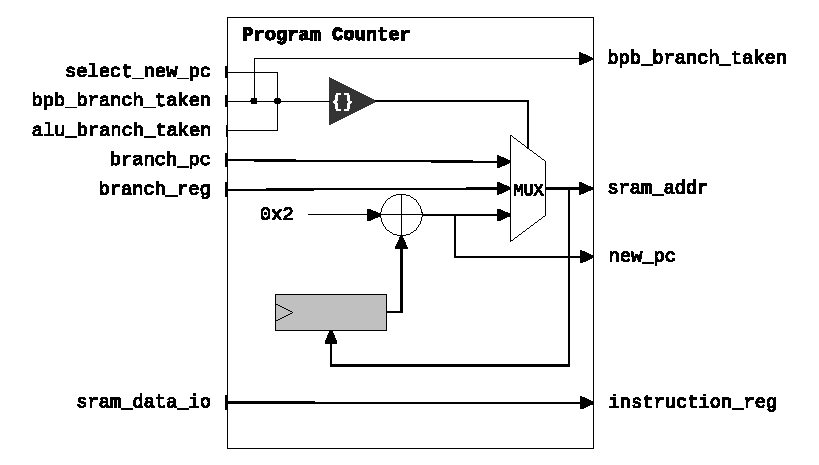
\includegraphics[width=\linewidth]{pictures/datapath/if_datapath.eps}
  \end{figure}   

  \newpage
  \subsection{Instruction Decode/Register Fetch}
  \subsubsection{Block Diagram}
  \begin{figure}[H]
    \centering
    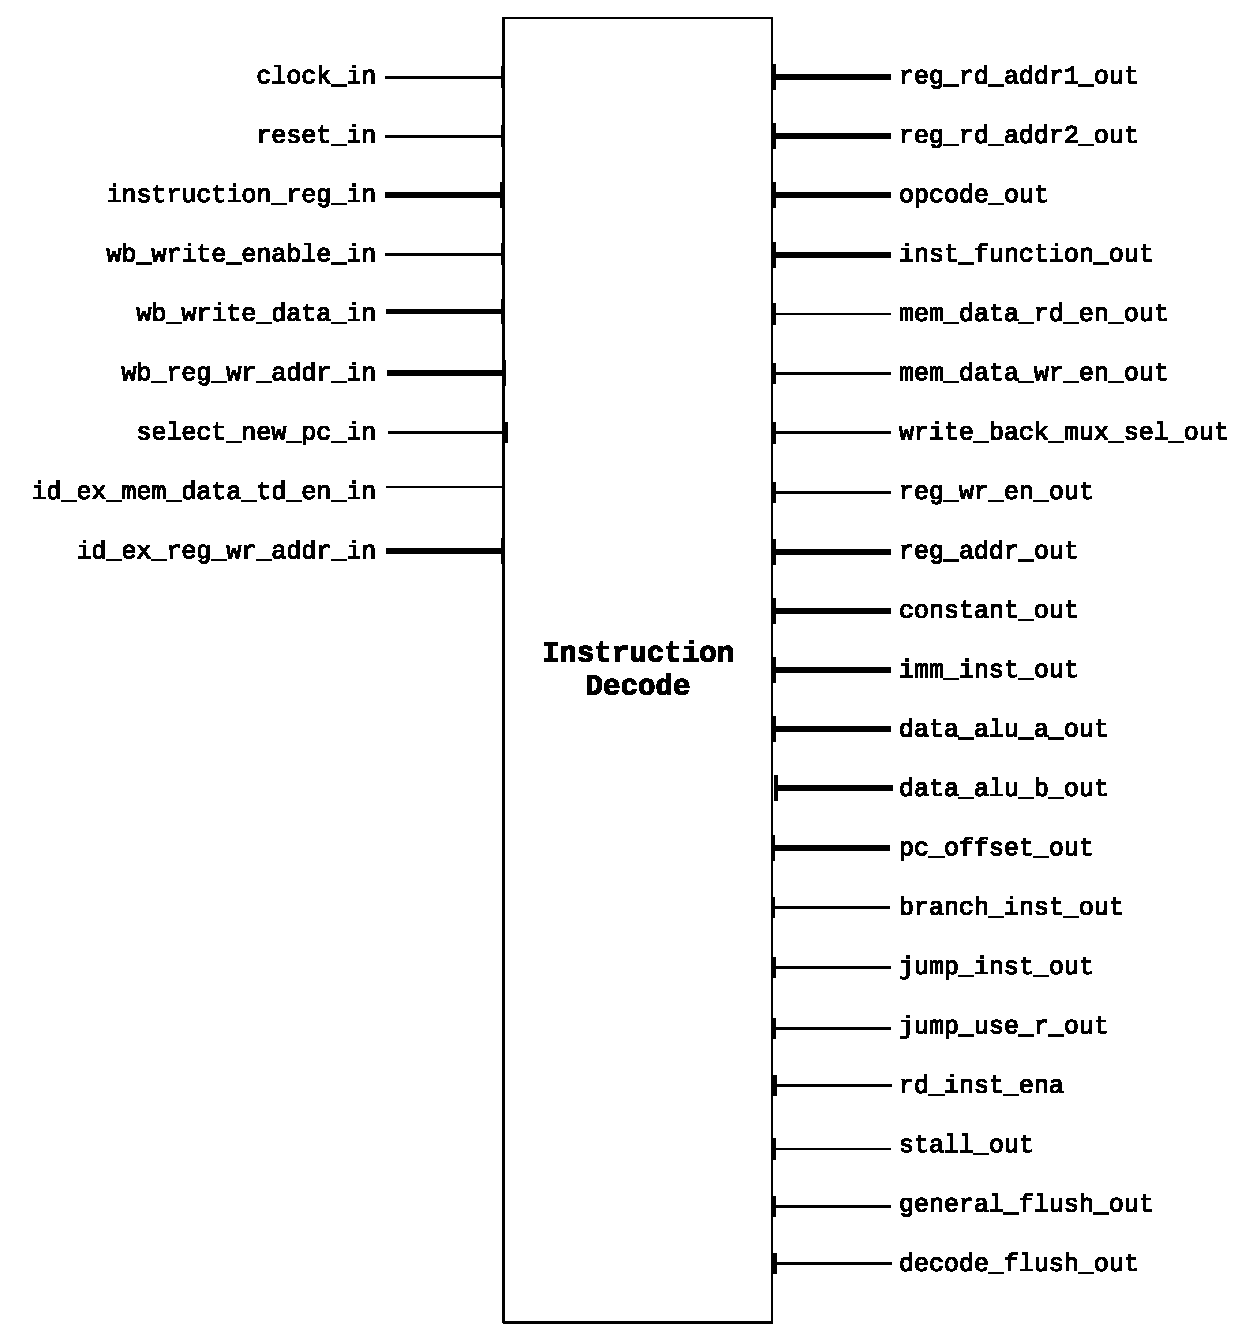
\includegraphics[width=.8\linewidth]{pictures/blocks/id_block.eps}
  \end{figure} 
  
  \subsubsection{Pin/Port Definitions}
  \FloatBarrier
    \begin{center}
      \begin{longtable}[pos]{| l | c | c | m{7cm} |} \hline       	
        \multicolumn{1}{|c|}{\cellcolor[gray]{0.9}\textbf{Name}} & 
        \multicolumn{1}{c|}{\cellcolor[gray]{0.9}\textbf{Length}} & 
        \multicolumn{1}{c|}{\cellcolor[gray]{0.9}\textbf{Direction}} &
        \multicolumn{1}{c|}{\cellcolor[gray]{0.9}\textbf{Description}} \\ \hline
        \endfirsthead
        \hline
        \multicolumn{4}{|l|}%
        {{\bfseries continued from previous page}} \\
        \hline
        \multicolumn{1}{|c|}{\cellcolor[gray]{0.9}\textbf{Name}} & 
        \multicolumn{1}{c|}{\cellcolor[gray]{0.9}\textbf{Length}} & 
        \multicolumn{1}{c|}{\cellcolor[gray]{0.9}\textbf{Direction}} &
        \multicolumn{1}{c|}{\cellcolor[gray]{0.9}\textbf{Description}} \\ \hline
        \endhead

        \hline \multicolumn{4}{|r|}{{continued on next page}} \\ \hline
        \endfoot

        \hline
        \endlastfoot

      	clock\_in 		          & 1 	& input 	& CPU core clock  	\\ \hline
      	reset\_in 		          & 1	  & input		& CPU core reset  	\\ \hline
      	instruction\_reg\_in    & 32	& input 	& CPU core instruction \\ \hline
      	new\_pc\_in 	          & 20	& input 	& Updated value of PC \\ \hline
      	alu\_src\_out 	            & 1	  & output 	& Alu mux source selector \\ \hline
      	alu\_opcode\_out 	      & 3	  & output 	& Alu opcode  \\ \hline
      	mem\_data\_wr\_en\_out 	        & 1	& output 	& Data memory write enable  \\ \hline
      	write\_back\_mux\_sel\_out 	    & 1	& output	  & Write back mux selector \\ \hline
      	w\_reg\_wr\_en\_out 	    & 1	& output 	& GPR bank write enable signal  \\ \hline
      	w\_reg\_addr\_out  & TBD   & output   & GPR bank destiny address \\ \hline
        constant\_out 	        & 32 & output 	& 32-bit Sign-extended constant  \\ \hline
        data\_alu\_a\_out    & 32   & output  & ALU input A data \\ \hline
        data\_alu\_b\_out & 32 & output & ALU input B data \\ \hline
        new\_pc\_out    & 20  & output  & Updated value of PC delayed  \\ \hline
        branch\_inst\_out         & 1  & output  & Conditional branch instruction  \\ \hline

        jmp\_inst\_out & 1 & output  & Incoditional branch instruction  \\ \hline
      \end{longtable}
    \end{center}
    
  \subsubsection{Internal Datapath} 
  The internal data path is composed by the following components.

  \begin{figure}[H]
    \centering
    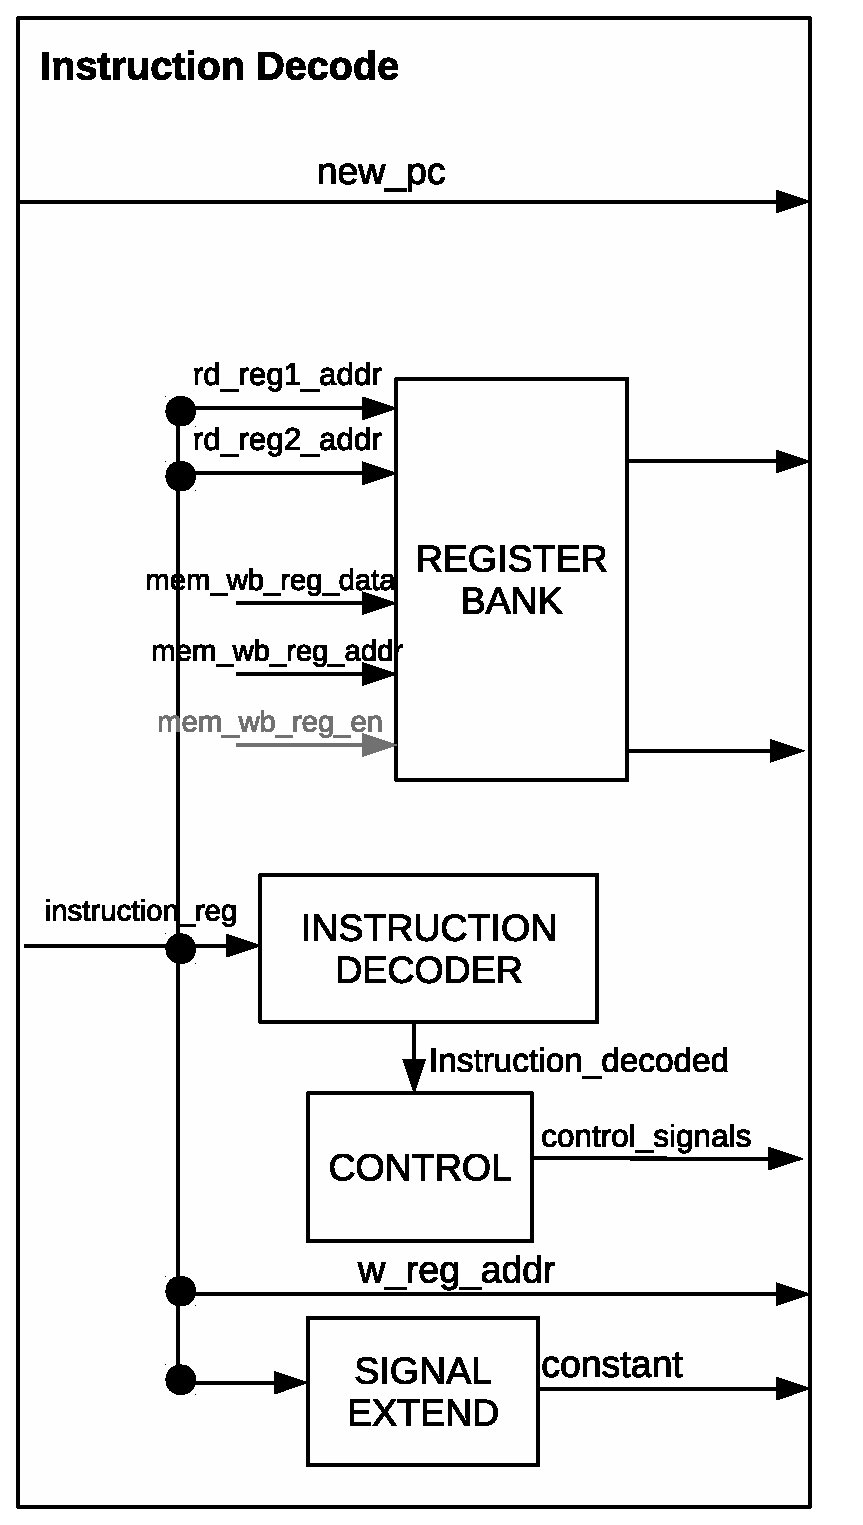
\includegraphics[width=0.45\linewidth]{pictures/datapath/id_datapath.eps}
  \end{figure} 
  
  
  \newpage
  \subsection{Execute/Address Calculate}
  \subsubsection{Block Diagram}
  \begin{figure}[H]
    \centering
    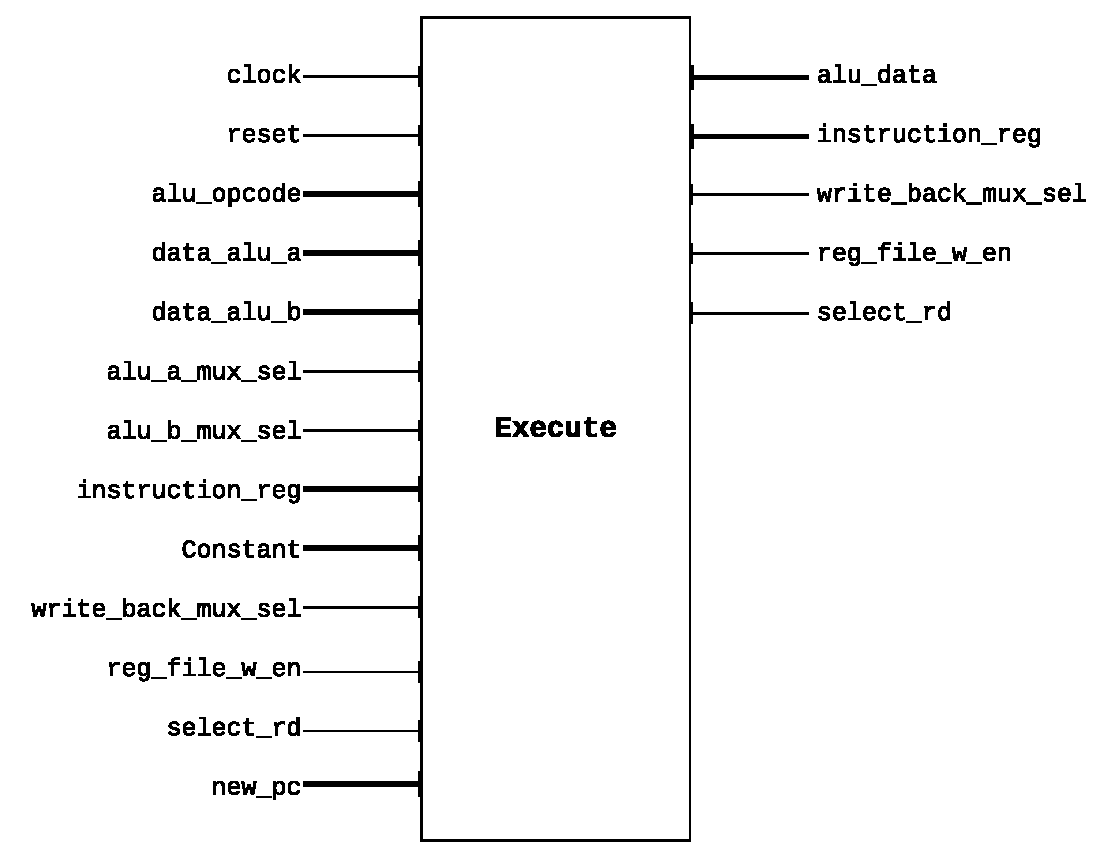
\includegraphics[width=\linewidth]{pictures/blocks/ex_block.eps}
  \end{figure} 

  \subsubsection{Pin/Port Definitions}
  \FloatBarrier
    \begin{center}
      \begin{longtable}[pos]{| l | c | c | m{7cm} |} \hline         
        \multicolumn{1}{|c|}{\cellcolor[gray]{0.9}\textbf{Name}} & 
        \multicolumn{1}{c|}{\cellcolor[gray]{0.9}\textbf{Length}} & 
        \multicolumn{1}{c|}{\cellcolor[gray]{0.9}\textbf{Direction}} &
        \multicolumn{1}{c|}{\cellcolor[gray]{0.9}\textbf{Description}} \\ \hline
        \endfirsthead
        \hline
        \multicolumn{4}{|l|}%
        {{\bfseries continued from previous page}} \\
        \hline
        \multicolumn{1}{|c|}{\cellcolor[gray]{0.9}\textbf{Name}} & 
        \multicolumn{1}{c|}{\cellcolor[gray]{0.9}\textbf{Length}} & 
        \multicolumn{1}{c|}{\cellcolor[gray]{0.9}\textbf{Direction}} &
        \multicolumn{1}{c|}{\cellcolor[gray]{0.9}\textbf{Description}} \\ \hline
        \endhead

        \hline \multicolumn{4}{|r|}{{continued on next page}} \\ \hline
        \endfoot

        \hline
        \endlastfoot

        clock\_in               & 1   & input   & CPU core clock    \\ \hline
        reset\_in               & 1   & input   & CPU core reset    \\ \hline
        alu\_src\_in            & ?? & input & ??? \\ \hline
        alu\_opcode\_in         & 3  & input  & ALU opperation code  \\ \hline        
        data\_alu\_a\_in        & 32 & input  & ALU input A data  \\ \hline
        data\_alu\_b\_in        & 32 & input  & ALU input B data  \\ \hline
        constant\_in            & 32 & input  & 32-bit Sign-extended constant  \\ \hline
        write\_back\_mux\_sel\_in & TBD & input & Write back mux select \\ \hline  
        w\_reg\_wr\_en\_in    & 1   & input  & GPR bank write enable \\ \hline 
        new\_pc\_in             & 20 & input  & Updated value of PC  \\ \hline 
        mem\_data\_wr\_en\_in & ?? & input & ??? \\ \hline
        w\_reg\_addr\_in & ?? & input & GPR bank destiny address \\ \hline
        branch\_inst\_in & ?? & input & ??? \\ \hline
		jmp\_inst\_in & ?? & input & ??? \\ \hline
		exe\_mem\_data\_in & ?? & input & ??? \\ \hline
		mem\_wb\_data\_in  & ?? & input & ??? \\ \hline 		
		mem\_data\_wr\_en\_out & 1 & output & ??? \\ \hline
        alu\_b\_data\_in\_out        & 32 & output  & ALU input B data  \\ \hline         
        alu\_data\_out           & 32  & output  & ALU data output \\ \hline
        write\_back\_mux\_sel\_out & TBD & output & Write back mux select \\ \hline  
        w\_reg\_wr\_en\_out    & 1   & output  & GPR bank write enable \\ \hline 
        w\_reg\_addr\_out & 4 & output & GPR bank destiny address \\ \hline
        branch\_inst\_out      & 1   & output  & Branch result after flag check \\ \hline
        alu\_zero\_out & 1 & output & ??? \\ \hline
        jmp\_inst\_out & 1 & output & ???\\ \hline

      \end{longtable}
    \end{center} 
     
  \subsubsection{Internal Datapath} 
  The internal data path is composed by the following components.

  \begin{figure}[H]
    \centering
    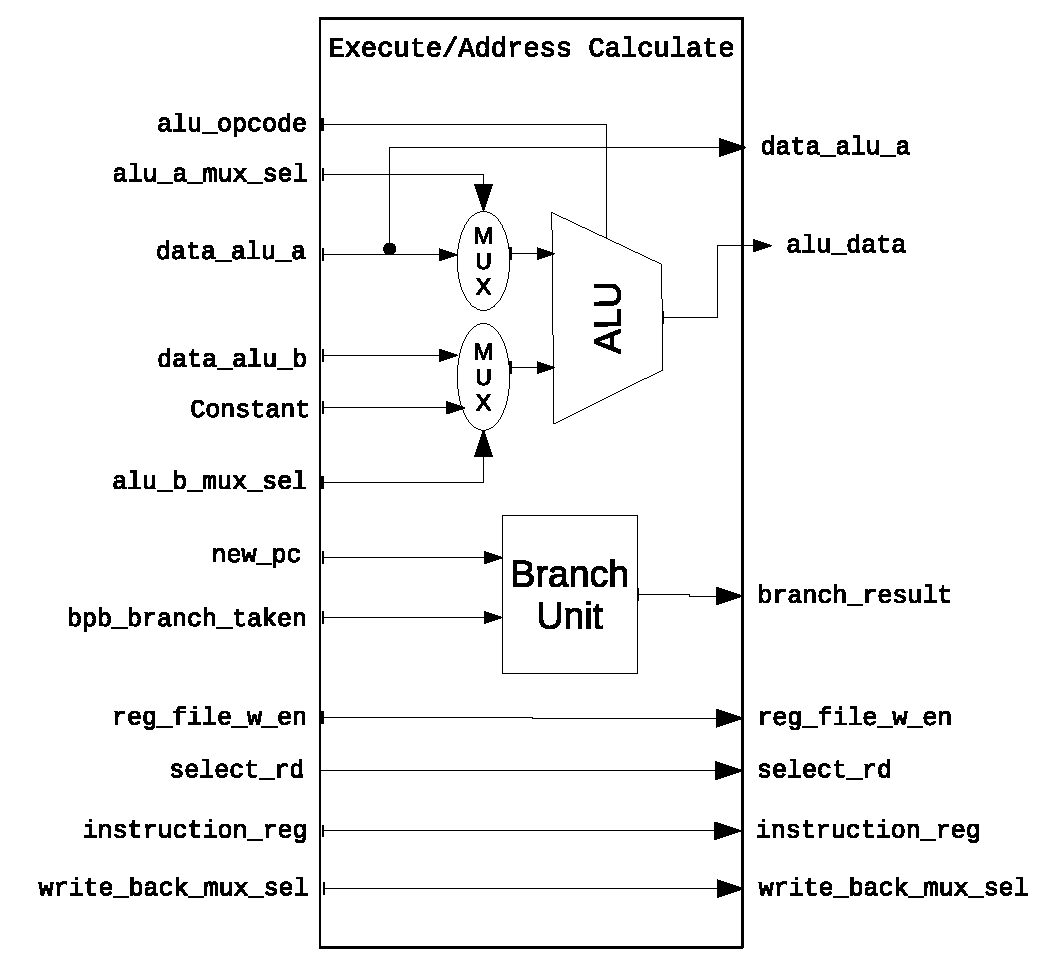
\includegraphics[width=.8\linewidth]{pictures/datapath/ex_datapath.eps}
  \end{figure}  

  \newpage
  \subsection{Memory Access}
  \subsubsection{Block Diagram}
  \begin{figure}[H]
    \centering
    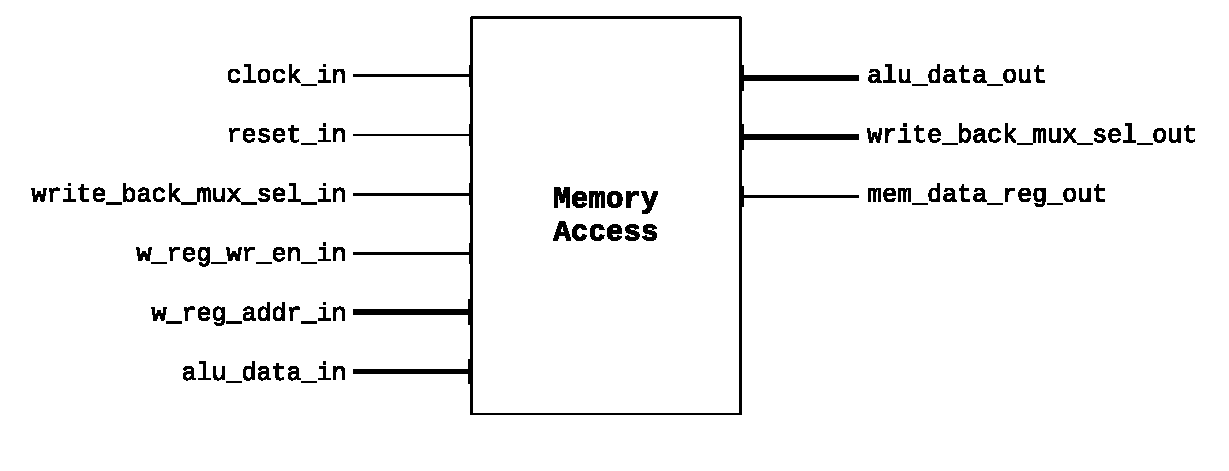
\includegraphics[width=\linewidth]{pictures/blocks/mem_block.eps}
  \end{figure} 

  \subsubsection{Pin/Port Definitions}
  \FloatBarrier
    \begin{center}
      \begin{longtable}[pos]{| l | c | c | m{7cm} |} \hline         
        \multicolumn{1}{|c|}{\cellcolor[gray]{0.9}\textbf{Name}} & 
        \multicolumn{1}{c|}{\cellcolor[gray]{0.9}\textbf{Length}} & 
        \multicolumn{1}{c|}{\cellcolor[gray]{0.9}\textbf{Direction}} &
        \multicolumn{1}{c|}{\cellcolor[gray]{0.9}\textbf{Description}} \\ \hline
        \endfirsthead
        \hline
        \multicolumn{4}{|l|}%
        {{\bfseries continued from previous page}} \\
        \hline
        \multicolumn{1}{|c|}{\cellcolor[gray]{0.9}\textbf{Name}} & 
        \multicolumn{1}{c|}{\cellcolor[gray]{0.9}\textbf{Length}} & 
        \multicolumn{1}{c|}{\cellcolor[gray]{0.9}\textbf{Direction}} &
        \multicolumn{1}{c|}{\cellcolor[gray]{0.9}\textbf{Description}} \\ \hline
        \endhead

        \hline \multicolumn{4}{|r|}{{continued on next page}} \\ \hline
        \endfoot

        \hline
        \endlastfoot

        clock\_in               & 1   & input  & CPU core clock    \\ \hline
        reset\_in               & 1   & input  & CPU core reset    \\ \hline
        write\_back\_mux\_sel\_in  & 1   & input  & Write back mux select \\ \hline        
        w\_reg\_wr\_en\_in        & 1   & input  & GPR bank write enable signal  \\ \hline        
        exe\_mem\_w\_reg\_addr         & TBD  & input  & GPR bank destiny address \\ \hline
        alu\_data\_in     & 32  & input  & ALU data output \\ \hline
        alu\_data\_out           & 32  & output  & ALU data output \\ \hline  
        write\_back\_mux\_sel\_out          & TBD & output  & Write back mux select \\ \hline                     
        mem\_wb\_w\_reg\_addr       & TBD & output & GPR bank destiny address \\ \hline

      \end{longtable}
    \end{center}  

  \subsubsection{Internal Datapath} 
  The internal data path is composed by the following components.

  \begin{figure}[H]
    \centering
    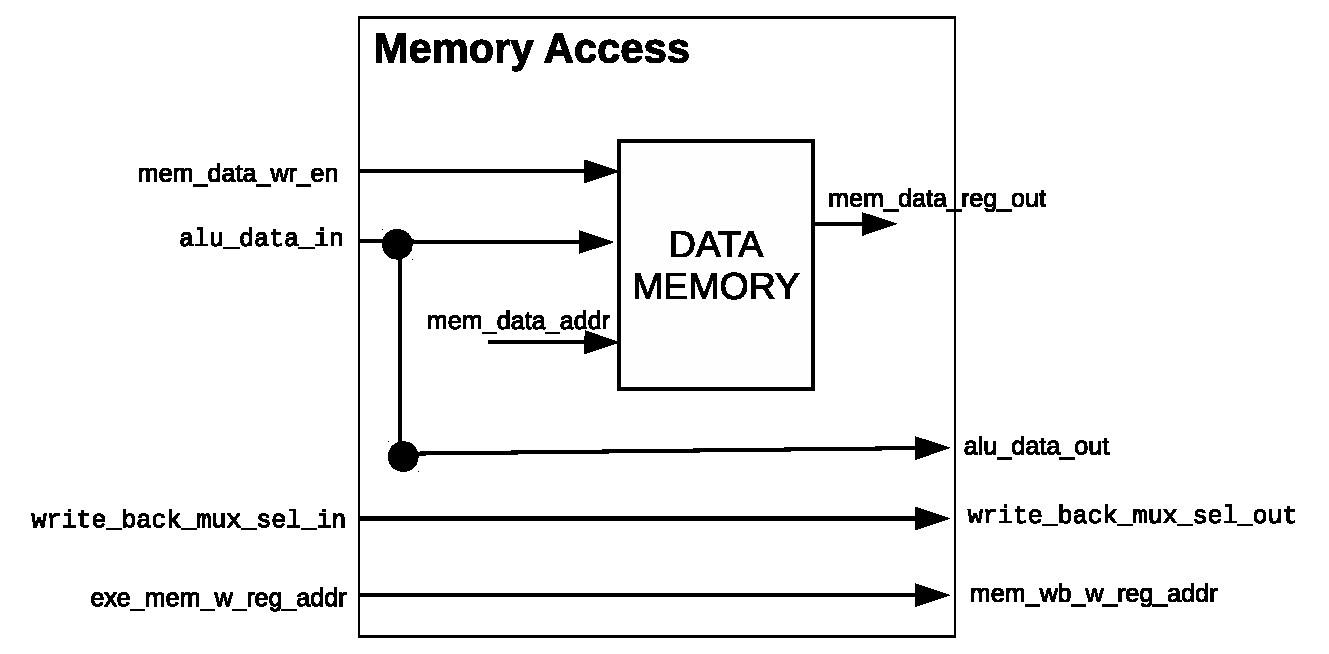
\includegraphics[width=.8\linewidth]{pictures/datapath/mem_datapath.eps}
  \end{figure}    
  
  \newpage
  \subsection{Write Back}
  \subsubsection{Block Diagram}
  \begin{figure}[H]
    \centering
    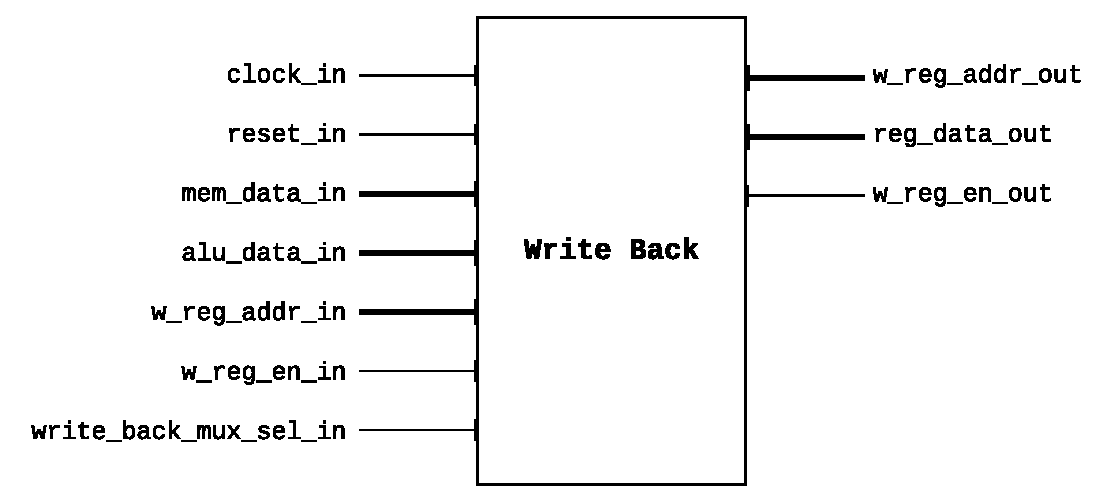
\includegraphics[width=\linewidth]{pictures/blocks/wb_block.eps}
  \end{figure} 

  \subsubsection{Pin/Port Definitions}
  \FloatBarrier
    \begin{center}
      \begin{longtable}[pos]{| l | c | c | m{7cm} |} \hline         
        \multicolumn{1}{|c|}{\cellcolor[gray]{0.9}\textbf{Name}} & 
        \multicolumn{1}{c|}{\cellcolor[gray]{0.9}\textbf{Length}} & 
        \multicolumn{1}{c|}{\cellcolor[gray]{0.9}\textbf{Direction}} &
        \multicolumn{1}{c|}{\cellcolor[gray]{0.9}\textbf{Description}} \\ \hline
        \endfirsthead
        \hline
        \multicolumn{4}{|l|}%
        {{\bfseries continued from previous page}} \\
        \hline
        \multicolumn{1}{|c|}{\cellcolor[gray]{0.9}\textbf{Name}} & 
        \multicolumn{1}{c|}{\cellcolor[gray]{0.9}\textbf{Length}} & 
        \multicolumn{1}{c|}{\cellcolor[gray]{0.9}\textbf{Direction}} &
        \multicolumn{1}{c|}{\cellcolor[gray]{0.9}\textbf{Description}} \\ \hline
        \endhead

        \hline \multicolumn{4}{|r|}{{continued on next page}} \\ \hline
        \endfoot

        \hline
        \endlastfoot

        clock\_in               & 1   & input  & CPU core clock    \\ \hline
        reset\_in               & 1   & input  & CPU core reset    \\ \hline
        mem\_data\_in           & 32  & input  & SDRAM data output \\ \hline
        alu\_data\_in           & 32  & input  & ALU data output \\ \hline
        w\_reg\_en\_in      & 4   & input  & GPR bank write enable signal \\ \hline
        w\_reg\_addr\_in        & 1   & input  & GPR bank destiny address  \\ \hline
        write\_back\_mux\_sel  & TBD & input  & Write back mux select  \\ \hline
        w\_reg\_addr\_out        & 4   & output & GPR bank destiny address  \\ \hline
        reg\_data\_out           & 32  & output & GPR bank write data  \\ \hline
        w\_reg\_en\_out    & 1  & output  & GPR bank write enable signal  \\ \hline
      \end{longtable}
    \end{center}  

  \subsubsection{Internal Datapath} 
  The internal data path is composed by the following components.

  \begin{figure}[H]
    \centering
    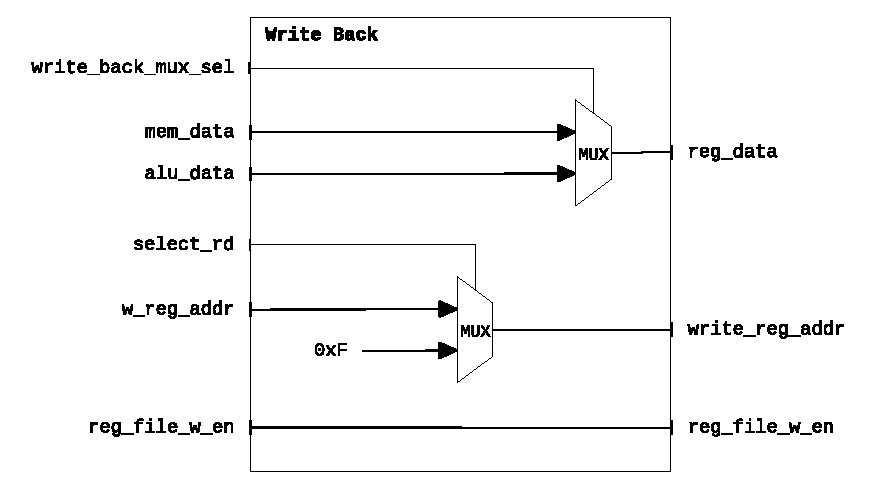
\includegraphics[width=\linewidth]{pictures/datapath/wb_datapath.eps}
  \end{figure}      
  
  \newpage
  \subsection{Pipeline Register Description}
  \subsubsection{Instruction Fetch/Instruction Decode}

  \FloatBarrier
    \begin{center}
      \begin{longtable}[pos]{| l | c | m{9cm} |} \hline         
        \multicolumn{1}{|c|}{\cellcolor[gray]{0.9}\textbf{Name}} & 
        \multicolumn{1}{c|}{\cellcolor[gray]{0.9}\textbf{Length}} & 
        \multicolumn{1}{c|}{\cellcolor[gray]{0.9}\textbf{Description}} \\ \hline
        \endfirsthead
        \hline
        \multicolumn{3}{|l|}%
        {{\bfseries continued from previous page}} \\
        \hline
        \multicolumn{1}{|c|}{\cellcolor[gray]{0.9}\textbf{Name}} & 
        \multicolumn{1}{c|}{\cellcolor[gray]{0.9}\textbf{Length}} & 
        \multicolumn{1}{c|}{\cellcolor[gray]{0.9}\textbf{Description}} \\ \hline
        \endhead

        \hline \multicolumn{3}{|r|}{{continued on next page}} \\ \hline
        \endfoot

        \hline
        \endlastfoot

        new\_pc           & 20  & Stores the next program counter value.\\ \hline
        instruction\_reg  & 32  & Stores the intruction word.    \\ \hline
        bpb\_branch\_taken       & 1   & Stores BPB result. \\ \hline

      \end{longtable}
    \end{center} 

  \subsubsection{Instruction Decode/Execute}

  \FloatBarrier
    \begin{center}
      \begin{longtable}[pos]{| l | c | m{9cm} |} \hline         
        \multicolumn{1}{|c|}{\cellcolor[gray]{0.9}\textbf{Name}} & 
        \multicolumn{1}{c|}{\cellcolor[gray]{0.9}\textbf{Length}} & 
        \multicolumn{1}{c|}{\cellcolor[gray]{0.9}\textbf{Description}} \\ \hline
        \endfirsthead
        \hline
        \multicolumn{3}{|l|}%
        {{\bfseries continued from previous page}} \\
        \hline
        \multicolumn{1}{|c|}{\cellcolor[gray]{0.9}\textbf{Name}} & 
        \multicolumn{1}{c|}{\cellcolor[gray]{0.9}\textbf{Length}} & 
        \multicolumn{1}{c|}{\cellcolor[gray]{0.9}\textbf{Description}} \\ \hline
        \endhead

        \hline \multicolumn{3}{|r|}{{continued on next page}} \\ \hline
        \endfoot

        \hline
        \endlastfoot

        new\_pc                 & 20  & Stores the next program counter value.\\ \hline
        data\_alu\_reg\_a       & 32  & Stores the value of ALU input port A.  \\ \hline
        data\_alu\_reg\_b       & 32  & Stores the value of ALU input port B. \\ \hline
        constant                & 32  & Stores the signed extended integer constant. \\ \hline
        instruction\_reg        & 32  & Stores the intruction word.    \\ \hline
        select\_rd\_reg           & 1   & TBD  \\ \hline
        reg\_file\_w\_en\_reg       & 1   & Stores the signal to enable GPR write back. \\ \hline
        write\_back\_mux\_sel\_reg  & TBD & Stores the select signal for write back Multiplexer. \\ \hline
        alu\_opcode              & 3   & Stores the ALU opperation code. \\ \hline
        select\_mux\_alu\_a        & TBD & Stores the ALU input data select signal \\ \hline
        select\_mux\_alu\_b        & TBD & Stores the ALU input data select signal \\ \hline
        bpb\_branch\_taken       & 1   & Stores BPB result. \\ \hline

      \end{longtable}
    \end{center} 

\subsubsection{Execute/Memory Access}

  \FloatBarrier
    \begin{center}
      \begin{longtable}[pos]{| l | c | m{9cm} |} \hline         
        \multicolumn{1}{|c|}{\cellcolor[gray]{0.9}\textbf{Name}} & 
        \multicolumn{1}{c|}{\cellcolor[gray]{0.9}\textbf{Length}} & 
        \multicolumn{1}{c|}{\cellcolor[gray]{0.9}\textbf{Description}} \\ \hline
        \endfirsthead
        \hline
        \multicolumn{3}{|l|}%
        {{\bfseries continued from previous page}} \\
        \hline
        \multicolumn{1}{|c|}{\cellcolor[gray]{0.9}\textbf{Name}} & 
        \multicolumn{1}{c|}{\cellcolor[gray]{0.9}\textbf{Length}} & 
        \multicolumn{1}{c|}{\cellcolor[gray]{0.9}\textbf{Description}} \\ \hline
        \endhead

        \hline \multicolumn{3}{|r|}{{continued on next page}} \\ \hline
        \endfoot

        \hline
        \endlastfoot

        instruction\_reg        & 32  & Stores the intruction word.    \\ \hline
        select\_rd\_reg         & 1   & TBD  \\ \hline
        reg\_file\_w\_en\_reg   & 1   & Stores the signal to enable GPR write back. \\ \hline
        write\_back\_mux\_sel\_reg  & TBD & Stores the select signal for write back Multiplexer. \\ \hline
        data\_alu\_a            & 32  & Stores the ALU input data A for memory addressing. \\ \hline
        alu\_data\_reg          & 32  & Stores the ALU output data. \\ \hline
      \end{longtable}
    \end{center}  

\subsubsection{Memory Access/Write Back}

  \FloatBarrier
    \begin{center}
      \begin{longtable}[pos]{| l | c | m{9cm} |} \hline         
        \multicolumn{1}{|c|}{\cellcolor[gray]{0.9}\textbf{Name}} & 
        \multicolumn{1}{c|}{\cellcolor[gray]{0.9}\textbf{Length}} & 
        \multicolumn{1}{c|}{\cellcolor[gray]{0.9}\textbf{Description}} \\ \hline
        \endfirsthead
        \hline
        \multicolumn{3}{|l|}%
        {{\bfseries continued from previous page}} \\
        \hline
        \multicolumn{1}{|c|}{\cellcolor[gray]{0.9}\textbf{Name}} & 
        \multicolumn{1}{c|}{\cellcolor[gray]{0.9}\textbf{Length}} & 
        \multicolumn{1}{c|}{\cellcolor[gray]{0.9}\textbf{Description}} \\ \hline
        \endhead

        \hline \multicolumn{3}{|r|}{{continued on next page}} \\ \hline
        \endfoot

        \hline
        \endlastfoot

        instruction\_reg        & 32  & Stores the intruction word.    \\ \hline
        select\_rd\_reg         & 1   & TBD  \\ \hline
        reg\_file\_w\_en\_reg   & 1   & Stores the signal to enable GPR write back. \\ \hline
        write\_back\_mux\_sel\_reg  & TBD & Stores the select signal for write back Multiplexer. \\ \hline
        mem\_data\_reg          & 32  & Stores the memory output data. \\ \hline
        alu\_data\_reg          & 32  & Stores the ALU output data. \\ \hline
        w\_reg\_addr\_reg       & 4   & Stores the GPR data write address. \\ \hline

      \end{longtable}
    \end{center}   

\newpage
  \subsection{Memory and Device Interface}
The memory and device interface is responsible for memory mapping to the processor. Depending on the address accessed a specific memory will be accessed by the memory device interface. If it is a read operation in the next clock cycle the read data will be directed to the DLX input read data port.

  \begin{figure}[H]
    \centering
    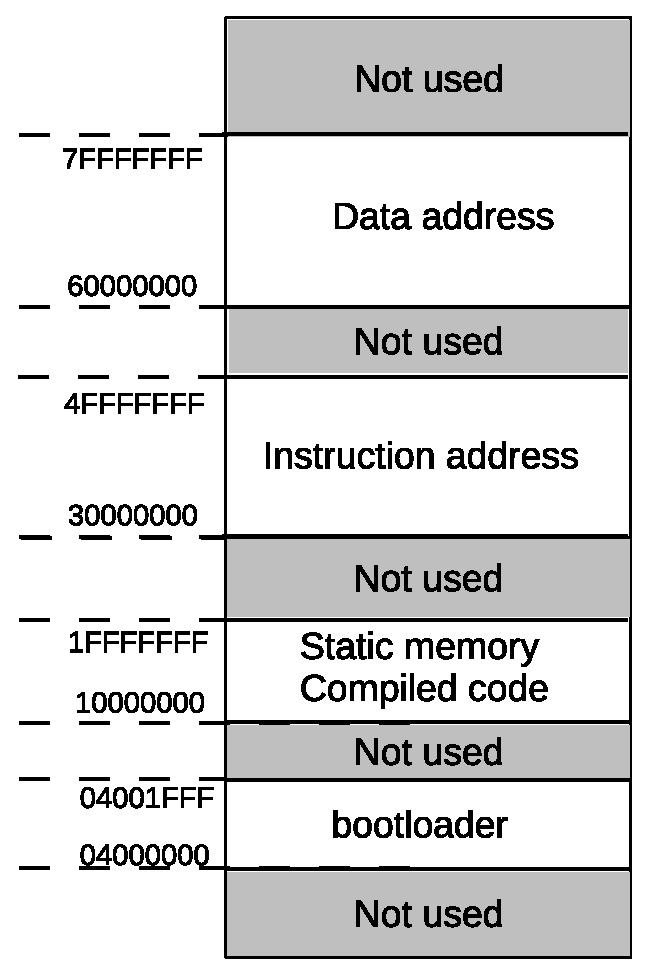
\includegraphics[width=0.4\linewidth]{pictures/mem_dev_interface.eps}
  \end{figure} 

The memory map shown was created with separate address to show that devices have no relation between them and to show that the memory used in this project will be a small fraction for the 4GBytes possible.

\newpage
  \subsection{SRAM Controller}
  The SRAM will store the instructions, as the SRAM has only 16 bits of word and an instruction has 32 bits the read and write operation must be done in a faster clock domain to avoid stopping the microprocessor.  
  The SRAM has instruction code this way this memory is not written in normal operation. The SRAM will be written by the processor just during the bootloader code is running and during this operation no read will be done. Not having read and write simultaneously make easier the control not needing to deal with write and read operations at the same time.
    \subsubsection{Block Diagram}
  \begin{figure}[H]
    \centering
    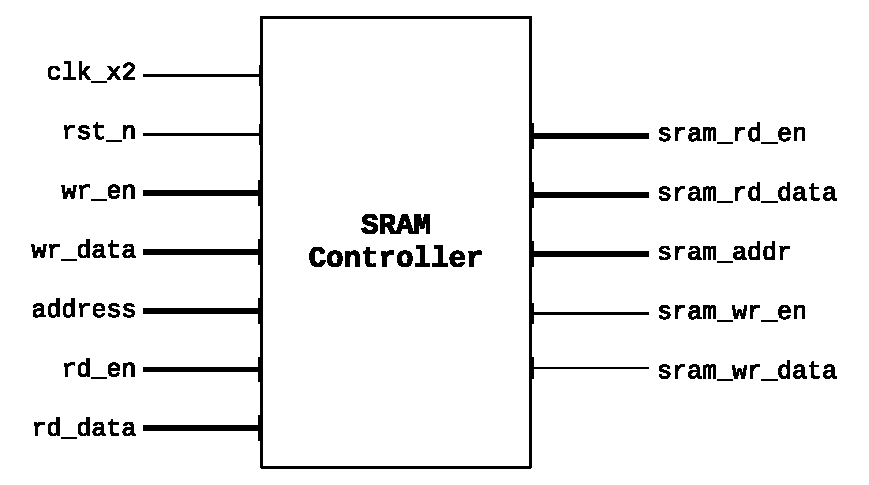
\includegraphics[width=.8\linewidth]{pictures/blocks/sram_block.eps}
  \end{figure}  

  \subsubsection{Pin/Port Definitions}
  \FloatBarrier
    \begin{center}
      \begin{longtable}[pos]{| l | c | c | m{7cm} |} \hline         
        \multicolumn{1}{|c|}{\cellcolor[gray]{0.9}\textbf{Name}} & 
        \multicolumn{1}{c|}{\cellcolor[gray]{0.9}\textbf{Length}} & 
        \multicolumn{1}{c|}{\cellcolor[gray]{0.9}\textbf{Direction}} &
        \multicolumn{1}{c|}{\cellcolor[gray]{0.9}\textbf{Description}} \\ \hline
        \endfirsthead
        \hline
        \multicolumn{4}{|l|}%
        {{\bfseries continued from previous page}} \\
        \hline
        \multicolumn{1}{|c|}{\cellcolor[gray]{0.9}\textbf{Name}} & 
        \multicolumn{1}{c|}{\cellcolor[gray]{0.9}\textbf{Length}} & 
        \multicolumn{1}{c|}{\cellcolor[gray]{0.9}\textbf{Direction}} &
        \multicolumn{1}{c|}{\cellcolor[gray]{0.9}\textbf{Description}} \\ \hline
        \endhead

        \hline \multicolumn{4}{|r|}{{continued on next page}} \\ \hline
        \endfoot

        \hline
        \endlastfoot

        clk\_x2               & 1   & input  & SRAM clock that is twice the DLX clock    \\ \hline
        rst\_n               & 1   & input  & System asynchronous reset    \\ \hline
        wr\_en           & 1  & input  & Data write enable \\ \hline
        wr\_data           & 32  & input  & Data to be written in the memory \\ \hline
        address      & 24   & input  & Memory address from the DLX \\ \hline
        rd\_en        & 1   & input  & Data read enable  \\ \hline
        rd\_data  & 32 & output  & Read data from SRAM to the DLX \\ \hline
        sram\_rd\_en          & 1 & output  & TBD \\ \hline
        sram\_rd\_data        & 16   & output & TBD  \\ \hline
        sram\_addr           & 10  & output & Memory address that goes to the SRAM  \\ \hline
        sram\_wr\_en    & 1  & output  & TBD  \\ \hline
        sram\_wr\_data    & 16  & output  & TBD  \\ \hline
      \end{longtable}
    \end{center} 
     
As the SRAM has half word the controller works with a clock twice faster enabling read two address, concatenating and sending to the DLX in time.

\newpage
  \subsection{SDRAM Controller}
  The SDRAM controller will be very simple and optimized to read or write one word that will be requested by the processor. There will be no burst, just one word write or read operation.
    \subsubsection{Block Diagram}
  \begin{figure}[H]
    \centering
    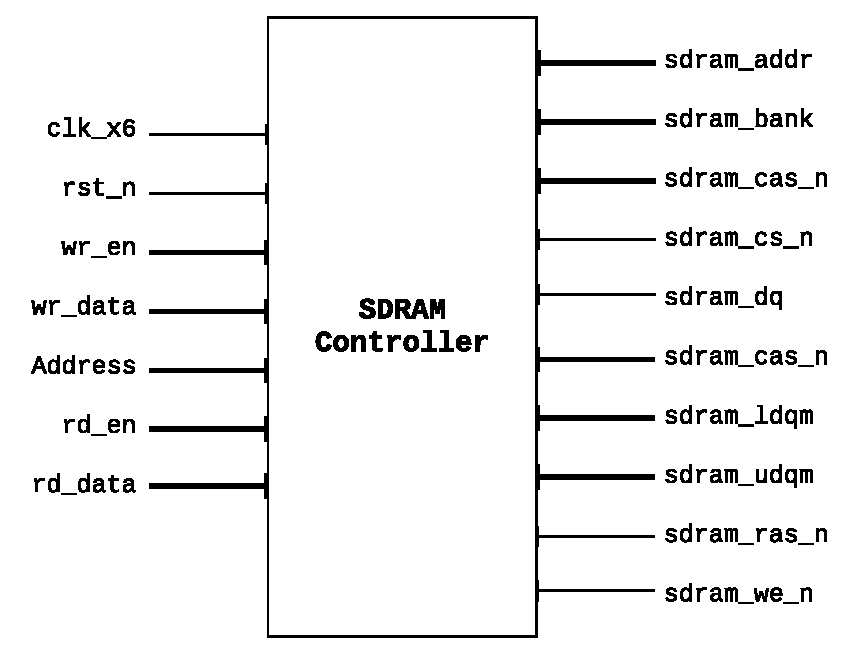
\includegraphics[width=\linewidth]{pictures/blocks/sdram_block.eps}
  \end{figure}  

  \subsubsection{Pin/Port Definitions}
  \FloatBarrier
    \begin{center}
      \begin{longtable}[pos]{| l | c | c | m{7cm} |} \hline         
        \multicolumn{1}{|c|}{\cellcolor[gray]{0.9}\textbf{Name}} & 
        \multicolumn{1}{c|}{\cellcolor[gray]{0.9}\textbf{Length}} & 
        \multicolumn{1}{c|}{\cellcolor[gray]{0.9}\textbf{Direction}} &
        \multicolumn{1}{c|}{\cellcolor[gray]{0.9}\textbf{Description}} \\ \hline
        \endfirsthead
        \hline
        \multicolumn{4}{|l|}%
        {{\bfseries continued from previous page}} \\
        \hline
        \multicolumn{1}{|c|}{\cellcolor[gray]{0.9}\textbf{Name}} & 
        \multicolumn{1}{c|}{\cellcolor[gray]{0.9}\textbf{Length}} & 
        \multicolumn{1}{c|}{\cellcolor[gray]{0.9}\textbf{Direction}} &
        \multicolumn{1}{c|}{\cellcolor[gray]{0.9}\textbf{Description}} \\ \hline
        \endhead

        \hline \multicolumn{4}{|r|}{{continued on next page}} \\ \hline
        \endfoot

        \hline
        \endlastfoot

        clk\_x6               & 1   & input  & SDRAM controller input clock. 6 times faster than DLX clock    \\ \hline
        rst\_n               & 1   & input  & System asynchronous reset    \\ \hline
        wr\_en           & 1  & input  & Data write enable \\ \hline
        wr\_data\_in           & 32  & input  & Data to be written in the memory \\ \hline
        address      & 24   & input  & Address of write or read operation \\ \hline
        rd\_en        & 1   & input  & Data read enable  \\ \hline
        rd\_data  & 32 & output  & Data read from the SDRAM to the memory interface \\ \hline
        sdram\_addr          & 12 & output  & SDRAM data address \\ \hline
        sdram\_bank        & 2   & output & The SDRAM selected Bank  \\ \hline
        sdram\_cas\_n           & 1  & output & SDRAM CAS  \\ \hline
        sdram\_cs\_n    & 1  & output  & SDRAM chip select  \\ \hline
        sdram\_dq    & 32  & output  & SDRAM read data, 2 bus of 16 bits, one for each memory  \\ \hline
        sdram\_ldqm    & 1  & output  & TBD  \\ \hline
        sdram\_udqm    & 1  & output  & TBD  \\ \hline
        sdram\_ras\_n    & 1  & output  & SRAM RAS  \\ \hline
        sdram\_we\_n    & 1  & output  & SDRAM write enable  \\ \hline
      \end{longtable}
    \end{center} 

% \newpage
%   \subsection{Forwarding Unit}
%   TBD in further releases.

\newpage  
  \subsection{Control Micro-instructions Description}
     \subsubsection{Block Diagram}
  \begin{figure}[H]
    \centering
    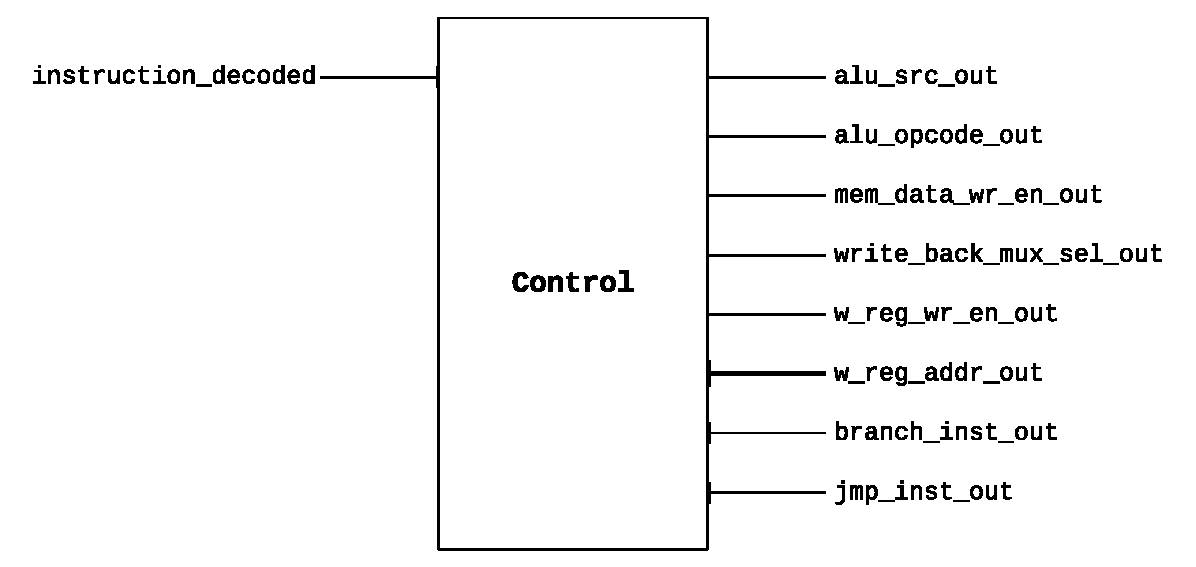
\includegraphics[width=\linewidth]{pictures/blocks/control_block.eps}
  \end{figure}  
  
    \subsubsection{Pin/Port Definitions}
  \FloatBarrier
    \begin{center}
      \begin{longtable}[pos]{| l | c | c | m{7cm} |} \hline         
        \multicolumn{1}{|c|}{\cellcolor[gray]{0.9}\textbf{Name}} & 
        \multicolumn{1}{c|}{\cellcolor[gray]{0.9}\textbf{Length}} & 
        \multicolumn{1}{c|}{\cellcolor[gray]{0.9}\textbf{Direction}} &
        \multicolumn{1}{c|}{\cellcolor[gray]{0.9}\textbf{Description}} \\ \hline
        \endfirsthead
        \hline
        \multicolumn{4}{|l|}%
        {{\bfseries continued from previous page}} \\
        \hline
        \multicolumn{1}{|c|}{\cellcolor[gray]{0.9}\textbf{Name}} & 
        \multicolumn{1}{c|}{\cellcolor[gray]{0.9}\textbf{Length}} & 
        \multicolumn{1}{c|}{\cellcolor[gray]{0.9}\textbf{Direction}} &
        \multicolumn{1}{c|}{\cellcolor[gray]{0.9}\textbf{Description}} \\ \hline
        \endhead

        \hline \multicolumn{4}{|r|}{{continued on next page}} \\ \hline
        \endfoot

        \hline
        \endlastfoot
        
        instruction\_decoded               & 1   & input  & TBD    \\ \hline
        alu\_src\_out\_n               & 1   & output  & TBD    \\ \hline
        alu\_opcode\_out           & 1  & output  & TBD \\ \hline
        mem\_data\_wr\_en\_out           & 1  & output  & TBD \\ \hline
        write\_back\_mux\_sel\_out      & 1   & output  & TBD \\ \hline
        w\_reg\_wr\_en\_out        & 1   & output  & TBD  \\ \hline
        w\_reg\_addr\_out  & 1 & output  & TBD \\ \hline
        branch\_inst\_out          & 12 & output  & TBD \\ \hline
        jmp\_inst\_out        & 1   & output & TBD  \\ \hline
        
      \end{longtable}
    \end{center} 
  
  \newpage
  \subsection{Bootloader}
  The bootloader is the ROM memory has the code responsible to initialize the processor and write the code that will be executed in the correct address and consequently each memory device.
The ROM must have the DLX reset PC register address. When the system is reseted the processor will read instructions from the ROM address. The code inside the ROM will copy the instruction and data code from a static memory to the instruction memory SRAM and the data memory SDRAM.

  \begin{figure}[H]
    \centering
    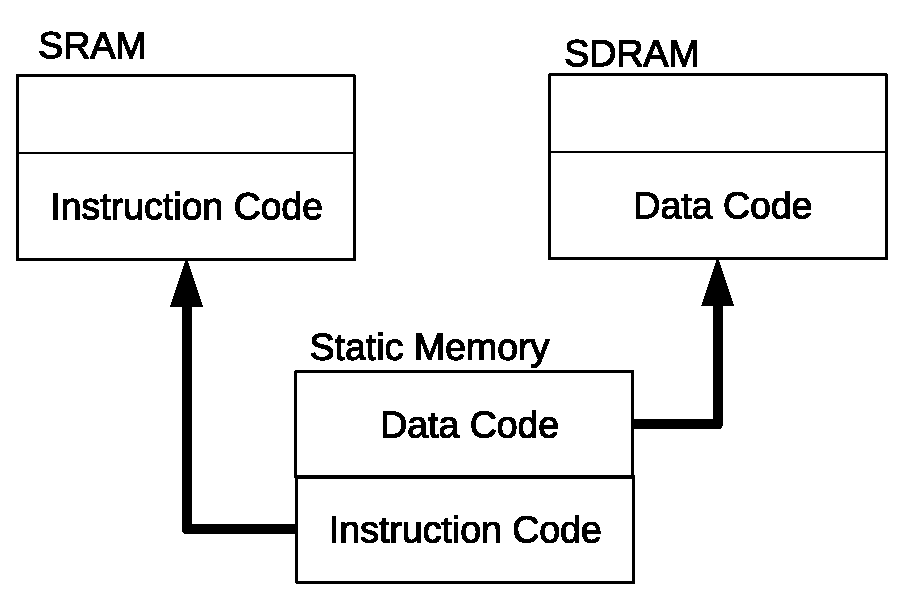
\includegraphics[width=.7\linewidth]{pictures/bootloader.eps}
  \end{figure}  
  Usually data in code is read-only data and it is common in compiled C code. Probably there will be only instruction code to be loaded during bootloader operation.
  
  
  %\newpage
  %\section{Timing}
    
% \bibliographystyle{ieeetr}
% \bibliography{ipprocess}

\end{document}
